\documentclass[11pt]{article}
\usepackage[a4paper,margin=25mm]{geometry}
\usepackage{amsmath,amssymb,amsthm,mathtools}
\usepackage[hidelinks,hypertexnames=false]{hyperref}
\usepackage{graphicx}
\usepackage{pdflscape}
\usepackage{mathrsfs}
\graphicspath{{figures/}{figures_029/}{figures_033/}{figures_finite_residue/}{figures_source_spectrum/}{figures_global_residue/}{figures_es_total/}{figures_prime_collision/}{figures_reciprocity_057/}{figures_factor_receiver_060/}{figures_period_continuation/}{figures_finite_period_064/}{figures_unit_phase_20260921/}{figures_real_pair_005/}{figures_real_pair_direction/}{figures_real_pair_local/}{./}}
\newtheorem{proposition}{Proposition}
\newtheorem{theorem}{Theorem}
\providecommand{\W}{\mathcal W}
\newcommand{\C}{\mathbb C}
\newcommand{\R}{\mathbb R}
\newcommand{\diag}{\operatorname{diag}}
\newcommand{\ord}{\operatorname{ord}}
\newcommand{\rank}{\operatorname{rank}}
\newcommand{\tr}{\operatorname{tr}}
\title{Two local branches and the exact conductor quotient}
\author{Split-Zero programme: coordinate calculation}
\date{21 September 2026}

\providecommand{\Spec}{\operatorname{Spec}}
\providecommand{\Disc}{\operatorname{Disc}}
\providecommand{\Tr}{\operatorname{Tr}}
\providecommand{\Span}{\operatorname{span}}

\providecommand{\im}{\operatorname{im}}
\providecommand{\Div}{\operatorname{div}}
\providecommand{\Tr}{\operatorname{Tr}}
\providecommand{\Hom}{\operatorname{Hom}}
\providecommand{\Res}{\operatorname{Res}}

\begin{document}\maketitle
\noindent Result SZ-20260921-008.  This reader gives the complete
RLA1--35 and RQT1--22 proofs.  The original certified point and
directional proofs are linked at their exact public editions and
included in the accompanying cumulative source and source archive.
All claims concern the stated geometric family.  The notation
$\alpha,\beta$ denotes its two spectral roots; the original unit
scale and quartet constant are explicitly distinguished below.
\tableofcontents\clearpage
\section{The complete local two-branch object and the original finite conductor}
\label{sec:real-pair-local-algebra}

This is a derivation for the certified member of the original geometric
family, with its original parameters recovered by exact inverse maps.
The point and full-series bounds are RPZ1--19 \cite{RPZ005};
the conjugation, old four-label return and finite reciprocal calculation
are RPCJ1--23, RPE1--26 and RPAC1--15
\cite{RPCJ005,RPE005,RPAC005}.
The companion complete directional source, RPD1--31 including RPD12a
\cite{RPD006,RPD31Source},
supplies the exact nonzero real Jacobian used below.  Its identity
RPD4 also follows directly from RPZ10--15, as recalled here.
The original matrix and Gamma frames are WCF1--6 \cite{WCF}, whose
\href{https://github.com/KokunoYumeto/zeta-function-research-reader/blob/5992ad50c0f2a06921f1fcaded7b4e38097c0739/workbenches/splitzero-tandem/continuations/20260920-original-kernel-mixed-determinants/providers/WEIGHTED_CONDUCTOR_FORWARD.tex#L28}{complete pinned proof}
retains the Meixner--Pollaczek provenance, DLMF
(18.19.8)--(18.19.9), (18.22.8), (18.23.7).
The original factor family is PCL1--10 \cite{PCLOriginal}, with its
\href{https://github.com/KokunoYumeto/zeta-function-research-reader/blob/487253b5b01851da5b9b98af4e146fecf1fab902/workbenches/splitzero-tandem/continuations/20260919-native-conductor-coprimality/providers/PCL_COMPLETE.tex#L19}{complete pinned proof}.
We prove the local constructions and all finite module identities below;
elementary analytic inversion, polynomial division and matrix elimination
are used with their proofs, not claimed as new general theorems.
The four marked states retain the canonical reader by The Clankers,
its theorem \texttt{explicit-four-time-Jacobian-collision}, and its
distinction between the antecedent three-dimensional example and the
four-dimensional marked construction \cite{ES488}.  The certified
interval arithmetic used in RPZ is Fredrik Johansson's Arb
\cite{human:arb2016}; the classical Gamma dictionary is
\cite{DLMF18Source}.  No arithmetic identification is made.

\subsection{Original functions, coefficient reflection and the exact parameter inverse}

Let $p=(z,x)$ and let $p_*=(z_*,x_*)$ be the unique real root in the
exact rational rectangle RPZ4.  Retain $u=1/z$, the four primary
exponents
\[
 \begin{gathered} (\rho_{\mathrm M}^{\rm prim},\rho_{\mathrm N}^{\rm prim},
 \rho_{\mathrm T}^{\rm prim},\rho_{\mathrm E}^{\rm prim})
 =(3/4+3i,3/4-3i,1/4+3i,1/4-3i),\\
 \delta=1/4,\quad\gamma=3,\quad\beta_0=143/8,\quad\eta=21025/256.
 \end{gathered}\tag{RLA1}
\]
The subscript on $\beta_0$ distinguishes this unchanged original
quartic constant from the spectral root $\beta(p)$ constructed below.
Likewise $\alpha_{\rm unit}$ denotes the unchanged nonzero real
scale written $\alpha$ in RPZ3: the actual unit remains
$a=\alpha_{\rm unit}(1+ix)$.
Put $w_a=\rho_a^{\rm prim}-1/2$, $V_{ar}=w_a^r$,
$J_d=\operatorname{diag}(1,-1,-1,1)$, $W(x)=I+ixJ_d$,
$\zeta=e^{2\pi i/5}$ and $D_j=\operatorname{diag}(\zeta^{-ja})_{a=1}^4$.
The complete original functions, with $1\le a\le4$, $0\le r\le3$, are
\[
\begin{aligned}
 \mathcal R(z)&=\sum_{n\ge0}R_nz^n,\\
 (R_n)_{ar}&=\sum_{\substack{h,k\ge0\\2h+4k=5n+r+1-a}}
 \frac{(\beta_0/3)^h\eta^k(-5)^{h+k-n}(a/5)_{h+k-n}}{h!k!},\\
 M_j(p)&=W(x)^{-1}V\mathcal R(z)^{-1}D_j\mathcal R(z)V^{-1}W(x),\\
 f_j(\xi,p)&=Q_0\bigl(M_j(p)(e^{\rho_a^{\rm prim}\xi})_a\bigr),\\
 Q_0(y)&=y_1y_4-y_2y_3,\\
 G(\xi,p)&=f_1(\xi,p)f_2(\xi,p),\\
 G^\#(\xi,p)&=\overline{G(\bar\xi,\bar p)},\\
 E_A(\xi,p)&=G(\xi,p)G^\#(\xi,p),\\
 g(t,p)&=e^{-4\omega(t)}E_A(\omega(t),p),\\
 \omega(t)&=-i\arctan t.
\end{aligned}\tag{RLA2}
\]
Empty sums are zero.  RPZ5--9 prove convergence, holomorphicity and
matrix invertibility on a complex neighborhood of $p_*$ after shrinking
it.  This last assertion also follows directly from the entire
convergence bound and nonzero determinants at $p_*$.
The reflection in RLA2 conjugates the Taylor coefficients in all three
variables.  It is holomorphic; it is not pointwise conjugation at a
complex parameter.  The real-coefficient series $\mathcal R$,
$\bar V=J_cV$, $\overline{W(\bar x)}=J_cW(x)J_c$, and
$Q_0(J_cy)=-Q_0(y)$ give $f_{5-j}=-f_j^\#$ identically.
Here $J_c$ exchanges indices $1,2$ and $3,4$.
Thus $G^\#=f_4f_3$ and the two minus signs cancel in $E_A$.
This proves the factor identity throughout the complex neighborhood.

All following derivatives without displayed arguments are at $(0,p_*)$.
Set $b_*=f_2\ne0$, $B=G_\xi\ne0$, $A_z=G_z$, $A_x=G_x$,
$b=|B|^2>0$ and
\[
 \begin{gathered}\Delta=\Im(\overline{A_z}A_x)\ne0,\qquad
 \mathcal H(p)=\binom{G(0,p)}{G^\#(0,p)},\\
 J_{\mathbb C}=D\mathcal H(p_*)=
 \begin{pmatrix}A_z&A_x\\\overline{A_z}&\overline{A_x}\end{pmatrix},
 \quad\det J_{\mathbb C}=-2i\Delta.
 \end{gathered}\tag{RLA3}
\]
The nonvanishing statement is proved, rather than assumed: RPZ12--13
give $\|I-PJ\|<1$ for the full real Jacobian
$J=D_p(\Re f_1,\Im f_1)$ and RPZ11 gives $\det P\ne0$.
The convergent geometric matrix series in $I-PJ$ inverts $PJ$,
so $J$ is invertible.  At the zero, multiplication by $b_*$ takes
$J$ to $D_p(\Re G,\Im G)$ and has determinant $|b_*|^2$.
Its determinant is precisely $\Delta$, proving RLA3.
The quantitative enclosure RPD31 has $\Delta<0$, but nonvanishing
alone suffices for the construction.

There is an actual holomorphic inverse $p=\mathcal P(r_+,r_-)$ to
$\mathcal H$, with
\[
 J_{\mathbb C}^{-1}
 =\frac1{-2i\Delta}
 \begin{pmatrix}\overline{A_x}&-A_x\\-\overline{A_z}&A_z\end{pmatrix},
 \qquad
 p_{n+1}=p_n-J_{\mathbb C}^{-1}
              \bigl(\mathcal H(p_n)-(r_+,r_-)^{\mathsf T}\bigr),
 \quad p_0=p_*.
 \tag{RLA4}
\]
To prove it, choose a closed complex ball about $p_*$ on which
$\|I-J_{\mathbb C}^{-1}D\mathcal H\|\le1/2$; continuity and RLA3
give such a ball.  Restrict $(r_+,r_-)$ so the displacement of its
center under RLA4 is at most one quarter of that ball's radius.
Integration along a segment gives a contraction ratio $1/2$ and
an image inside three quarters of the radius.  The differences of
successive iterates are bounded by a geometric series.  The uniform
limit exists and is the unique fixed point, hence exactly a solution
of $\mathcal H(p)=(r_+,r_-)$.
Every iterate is holomorphic in the parameters; local uniform
convergence and the coefficientwise Cauchy integral formula show that
the limit is holomorphic.  Uniqueness proves both inverse compositions
after restriction to these neighborhoods.  In particular all original
coordinates are recovered, with $u=1/\mathcal P_z$ and
$a=\alpha_{\rm unit}(1+i\mathcal P_x)$, without identifying a scale
or an original parameter with a chosen constant.

Since $g(0,p)=r_+r_-$, its zero divisor is the union of the two
smooth curves $r_+=0$ and $r_-=0$, meeting transversely only at $p_*$.
Each factor has multiplicity one.  On the real parameter slice
$r_-=\overline{r_+}$, so their union meets that slice only at $p_*$.
This is the complete local zero divisor of the original zeroth
moment, not only its tangent cone.

\subsection{The two actual spectral roots and their full analytic units}

Put $F_+(t,p)=G(\omega(t),p)$ and
$F_-(t,p)=G^\#(\omega(t),p)$.
Their $t$ derivatives at the base point are $-iB$ and
$-i\bar B$, respectively, both nonzero.  There are unique
holomorphic roots $\alpha(p),\beta(p)$ close to zero, given by the
convergent iterations
\[
\begin{aligned}
 t^+_{n+1}&=t^+_n-F_+(t^+_n,p)/(-iB),&t^+_0&=0,\\
 t^-_{n+1}&=t^-_n-F_-(t^-_n,p)/(-i\bar B),&t^-_0&=0,\\
 \alpha(p)&=\lim_nt^+_n,&\beta(p)&=\lim_nt^-_n.
\end{aligned}\tag{RLA5}
\]
The proof is the one-dimensional version of RLA4: on a sufficiently
small fixed complex disk and parameter neighborhood each derivative
of the iteration in its first variable has modulus at most $1/2$,
and its value at zero has modulus at most one quarter of the radius.
The same geometric and Cauchy integral arguments give unique
holomorphic limits.  Consequently these are roots of the actual
infinite-series factors.  Because $f_2$ and $f_3$ stay nonzero, they
are exactly the roots of the original $f_1$ and $f_4$, respectively.
The original spectral coordinates are
$\xi_+=\omega(\alpha)$ and $\xi_-=\omega(\beta)$; the inverse
spectral morphism is $t=\tan(i\xi)=i\tanh\xi$ on this neighborhood.
Multiplication of its derivative by $\omega'(t)$ and the values at
zero, or the defining arctangent identity, verifies both compositions.

The complete units and complete factorization are
\[
\begin{aligned}
 U_+(t,p)&=\int_0^1\partial_tF_+
       (\alpha(p)+\theta(t-\alpha(p)),p)\,d\theta,\\
 U_-(t,p)&=\int_0^1\partial_tF_-
       (\beta(p)+\theta(t-\beta(p)),p)\,d\theta,\\
 F_+&=(t-\alpha)U_+,&F_-&=(t-\beta)U_-,\\
 U(t,p)&=e^{-4\omega(t)}U_+(t,p)U_-(t,p),&
 q(t,p)&=(t-\alpha)(t-\beta),\\
 g(t,p)&=U(t,p)q(t,p),&U(0,p_*)&=-|B|^2=-b.
\end{aligned}\tag{RLA6}
\]
Integration of the derivative proves both divisions exactly.
Integration of locally convergent Taylor series proves the units
holomorphic; their values at the base point are $-iB$ and
$-i\bar B$.  They, their product, and the center exponential are
nonzero on a smaller neighborhood.  No coefficient of any unit
has been removed.  In particular
\[
 r_+=-\alpha U_+(0,p),\qquad r_-=-\beta U_-(0,p),\qquad
 g_0=U(0,p)\alpha\beta.
 \tag{RLA7}
\]
Thus $\alpha=0$ and $\beta=0$ are precisely the two original
parameter branches, with the original $r_\pm$ factors retained.

The roots themselves are a pair of holomorphic coordinates.  Implicit
differentiation of the two proved zero equations gives
\[
 D\alpha(p_*)=-\frac{i}{B}(A_z,A_x),\qquad
 D\beta(p_*)=-\frac{i}{\bar B}(\bar A_z,\bar A_x),\qquad
 \det D(\alpha,\beta)(p_*)=\frac{2i\Delta}{b}\ne0.
 \tag{RLA8}
\]
An exact inverse, not just the derivative, is constructed as follows.
For proposed roots $(A_0,B_0)$ close to zero iterate
\[
 p_{n+1}=p_n-J_{\mathbb C}^{-1}
       \binom{F_+(A_0,p_n)}{F_-(B_0,p_n)},\qquad p_0=p_*.
 \tag{RLA9}
\]
Its parameter derivative vanishes at $(A_0,B_0,p)=(0,0,p_*)$.
The ball argument of RLA4 proves a unique holomorphic limit
$p=\mathcal P_{\rm roots}(A_0,B_0)$.
Uniqueness in RLA5 then proves
\[ (\alpha,\beta)(\mathcal P_{\rm roots}(A_0,B_0))=(A_0,B_0). \]
The other inverse composition follows from uniqueness in RLA9.
This explicitly restores $z,x,u,a$ from the spectral-root coordinates.

For a parameter function write $h^\sharp(p)=\overline{h(\bar p)}$.
Since $\overline{\omega(-\bar t)}=\omega(t)$, the exact reflection
and real-slice restrictions are
\[
 F_-(t,p)=\overline{F_+(-\bar t,\bar p)},\qquad
 \beta=-\alpha^\sharp,\qquad
 U(-\bar t,\bar p)=\overline{U(t,p)},\qquad
 \beta(p)=-\overline{\alpha(p)}\quad(p\in\mathbb R^2).
 \tag{RLA10}
\]
The first identity and uniqueness in RLA5 prove the second.
Reflecting both linear factors in RLA6, including their minus signs,
proves the identity for $U$.  On the real slice $U(0,p)$ is real
and stays negative, since its value at $p_*$ is $-b$.
Accordingly $g_0=-U(0,p)|\alpha(p)|^2>0$ away from $p_*$.
The spectral collision curve $\alpha=\beta$ is a different curve
from the parameter branches $\alpha=0$, $\beta=0$.
At its nonzero points $g_0\ne0$, so collision of the two nonzero
spectral roots does not make the finite conductor singular.

\subsection{Every cutoff and the full two-generator module}

Let $R$ be the local ring of convergent holomorphic parameter germs
at $p_*$.  RLA9 gives mutually inverse ring identifications
$R\simeq\mathbb C\{\alpha,\beta\}$; the original parameter maps and
unit remain those already displayed.  Put $\sigma=\alpha+\beta$,
$\pi=\alpha\beta$, $R_N=R[t]/(t^N)$ for $N\ge1$ and
$q=t^2-\sigma t+\pi$.  Write $L_N(h)$ for multiplication by the
full series $h$ modulo $t^N$ in the ordered basis $1,t,\ldots,t^{N-1}$.
Each entry uses the exact coefficient, not a truncated substitute
for that coefficient.  Since $U(0,p)$ is a unit, the finite inverse
of $L_N(U)$ is multiplication by $U^{-1}$ modulo $t^N$; its
coefficients are specified recursively by
\[
 \begin{gathered}v_0=U_0^{-1},\qquad
 v_n=-U_0^{-1}\sum_{j=1}^nU_jv_{n-j},\\
 L_N(g)=L_N(q)L_N(U),\qquad
 \mathcal M_N:=\operatorname{coker}L_N(g)=R[t]/(t^N,q).
 \end{gathered}\tag{RLA11}
\]
Here $U_j=[t^j]U$, and the equality of cokernels uses the identity on
the target: $(g)=(q)$ in $R_N$, because multiplication by $U$ is
invertible there.  The corresponding source morphism is $L_N(U)$
and its exact inverse is the displayed recurrence.  Its metric
effect is calculated below, rather than declared isometric.

Define $h_{-1}=0$, $h_0=1$ and
\[
 h_n(\alpha,\beta)=\sum_{j=0}^n\alpha^{n-j}\beta^j\quad(n\ge0),
 \qquad h_n=\sigma h_{n-1}-\pi h_{n-2}\quad(n\ge1),\qquad
 C=\begin{pmatrix}0&-\pi\\1&\sigma\end{pmatrix}.
 \tag{RLA12}
\]
The recurrence for $n=1$ means $h_1=\sigma$; for $n\ge2$ it
follows by multiplying and cancelling the finite sums.
Polynomial division by the monic $q$ is exact over $R$ and leaves
a unique representative $a+bt$.  Indeed each power $t^n$ with
$n\ge2$ is reduced using $t^2=\sigma t-\pi$, and a nonzero
multiple of the monic quadratic has degree at least two.
Multiplication by $t$ on this rank-two module has the matrix $C$.
Induction gives the complete remainders
\[
 [t^n]_q=-\pi h_{n-2}+h_{n-1}t\quad(n\ge1),\qquad
 C^N=\begin{pmatrix}
 -\pi h_{N-2}&-\pi h_{N-1}\\h_{N-1}&h_N
 \end{pmatrix}\quad(N\ge1).
 \tag{RLA13}
\]
The first formula at $n=1$ uses $h_{-1}=0$.
The columns of $C^N$ are exactly the remainders of $t^N,t^{N+1}$.
Every multiple of $t^N$ in $R[t]/q$ is their $R$-linear combination,
since that ring has basis $1,t$.  Hence the full conductor has the
two-generator presentation
\[
 R^2\xrightarrow{\ C^N\ }R^2\longrightarrow\mathcal M_N
 \longrightarrow0,\qquad
 [a+bt]\longmapsto[a+bt]\bmod(t^N,q).
 \tag{RLA14}
\]
The inverse to its cokernel map reduces any polynomial modulo $q$
by RLA13.  Reducing a multiple of $t^N$ changes its remainder by
$C^N$ times a vector, and reducing a multiple of $q$ changes it by
zero.  These facts prove well-definedness and both compositions.
Conversely, a remainder in the image of $C^N$ is a multiple of
$t^N$ modulo $q$, so the same argument proves injectivity.
Thus RLA14 describes the entire module, not only its dimension at
the special point.  It includes $N=1$: the unit entry of $C$ leaves
$\mathcal M_1=R/(\pi)$.

In the displayed presentation the determinant and entry ideals are
\[
 \operatorname{Fitt}_0(\mathcal M_N)=(\pi^N),\qquad
 \operatorname{Fitt}_1(\mathcal M_N)
   =(h_{N-1},\pi h_{N-2}),\qquad
 \operatorname{Fitt}_j(\mathcal M_N)=R\quad(j\ge2).
 \tag{RLA15}
\]
Here Fitting ideals mean the ideals of minors of sizes two, one
and zero in RLA14.  The determinant is $(\det C)^N=\pi^N$;
$h_N=\sigma h_{N-1}-\pi h_{N-2}$ gives the entry ideal.
For $N=1$ it is $R$, since $h_0=1$.
These are also the corresponding ideals from the original
$N$-generator presentation: adding a generator with a relation that
solves uniquely for it, or eliminating such a pair, adjoins or removes
an identity block.  The minors of that enlarged block give precisely
the same ideals with their shifted sizes.  Multiplication of a
presentation by invertible matrices leaves its minors' ideals fixed
by the determinant expansion, applied also to the inverse matrices.
For an explicit common presentation start with generators
$1,t,\ldots,t^{N+1}$ and relations
$q,tq,\ldots,t^{N-1}q,t^N,t^{N+1}$.
Eliminating the last two generators with their unit-coefficient
relations gives the original multiplication-by-$q$ presentation
modulo $t^N$.  Instead eliminating $t^2,\ldots,t^{N+1}$ in order
with the first $N$ monic relations leaves $1,t$ and precisely the
two columns of $C^N$.  These are the indicated invertible
generator and relation operations; no ideal is inferred from
dimensions alone.
For $N\ge2$ the common zero of the two generators of
$\operatorname{Fitt}_1$ near the origin is just $\alpha=\beta=0$:
if $\pi=0$ and one root is nonzero, $h_{N-1}$ is its nonzero
$(N-1)$st power; if $\pi\ne0$, consecutive $h$'s cannot both vanish,
as the recurrence backwards would force $h_0=0$.

\subsection{The exact gluing of the two branches}

Evaluation at the two roots is an injective map on $R[t]/q$:
\[
 a+bt\longmapsto(a+b\alpha,a+b\beta),\qquad
 \mathcal L=\{(v_+,v_-)\in R^2:
                      v_+-v_-\in(\alpha-\beta)\}.
 \tag{RLA16}
\]
Its image is exactly $\mathcal L$: divide $v_+-v_-$ by
$\alpha-\beta$ to recover $b$, and then set $a=v_+-b\alpha$.
Its kernel is zero since $(\alpha-\beta)b=0$ in the integral
domain of convergent series.  Multiplication by $t^N$ becomes
$\operatorname{diag}(\alpha^N,\beta^N)$ on this lattice.
It follows, with all maps specified, that
\[
\begin{gathered}
 0\longrightarrow\mathcal M_N
 \xrightarrow{\,\iota\,}R/(\alpha^N)\oplus R/(\beta^N)
 \xrightarrow{\,d\,}R/(\alpha-\beta,\alpha^N)
 \longrightarrow0,\\
 \iota([P])=(P(\alpha)\bmod\alpha^N,
                         P(\beta)\bmod\beta^N),\qquad
 d([v_+],[v_-])=[v_+-v_-].
\end{gathered}\tag{RLA17}
\]
The last map is well defined and onto.  Its kernel consists of
pairs whose representatives differ by an element of
$(\alpha-\beta,\alpha^N)$; changing the first representative by
a multiple of $\alpha^N$ puts them in $\mathcal L$, proving that
the kernel is the image of $\iota$.
For injectivity, suppose $(\alpha^Nr,\beta^Ns)\in\mathcal L$.
Modulo $\alpha-\beta$ the relation is
$\alpha^N(r-s)=0$ in $\mathbb C\{\alpha\}$.
This ring is a domain, so $r-s$ is divisible by $\alpha-\beta$.
Thus $(r,s)\in\mathcal L$, and the original pair is a multiple of
$t^N$ in the lattice, proving that its class is zero.
This proves exactness directly, including the intersection coupling.
The gluing quotient has complex dimension $N$, with basis
$1,\alpha,\ldots,\alpha^{N-1}$ after setting $\beta=\alpha$.
The module is not the direct sum of the two branch modules for
any $N\ge1$.  For $N=1$ its minimal generator count is one,
whereas that direct sum needs two, as reduction modulo
$(\alpha,\beta)$ shows.  For $N\ge2$, RLA15's first Fitting
ideal contains $h_{N-1}$, a nonzero homogeneous polynomial of
degree $N-1$.  The first Fitting ideal of the diagonal
presentation of $R/(\alpha^N)\oplus R/(\beta^N)$ is
$(\alpha^N,\beta^N)$; every element has order at least $N$.
Those ideals differ, so the presentation invariance just proved
excludes an isomorphism.  RLA17 retains the exact embedding and
gluing map that relates these modules.

The annihilator is exactly
\[
 \operatorname{Ann}_R(\mathcal M_N)
       =(\alpha^N)\cap(\beta^N)=(\alpha^N\beta^N).
 \tag{RLA18}
\]
Injection in RLA17 gives inclusion from right to left.
Each projection of $\iota$ is onto, because constant polynomials
give every residue in each component; hence an annihilator must
lie in both ideals.  In the convergent double Taylor series,
divisibility by $\alpha^N$ removes all powers of $\alpha$ below
$N$, and divisibility by $\beta^N$ removes all powers of $\beta$
below $N$.  Both together give divisibility by their product.
At a point of $\alpha=0$ with $\beta\ne0$, the second branch
module and the gluing quotient in RLA17 vanish locally, so the
module is exactly $R/(\alpha^N)$ there.  The corresponding
statement on the other branch is $R/(\beta^N)$.
At their intersection, RLA14 reduced modulo $(\alpha,\beta)$ has
zero matrix for $N\ge2$, and therefore a two-dimensional fiber.
For $N=1$ the fiber has dimension one, as already calculated.
The two dimensions at the intersection record the two original
lost directions; the gluing map retains how the branches approach
that intersection.

\subsection{Exact connection to the directional resonances and the full inverse}

Away from $\alpha\beta=0$ the exact inverse coefficients are
\[
 [t^n]\frac1{g(t,p)}
 =\sum_{j=0}^n v_j(p)
       \frac{h_{n-j}(\alpha(p),\beta(p))}
            {(\alpha(p)\beta(p))^{n-j+1}},\qquad 0\le n<N,
 \tag{RLA19}
\]
where every $v_j$ is the full unit reciprocal from RLA11.
Indeed the geometric expansions of $(t-\alpha)^{-1}$ and
$(t-\beta)^{-1}$ yield
$[t^m]q^{-1}=h_m(\alpha,\beta)/(\alpha\beta)^{m+1}$.
Finite convolution with $U^{-1}$ proves RLA19.  It holds also
when $\alpha=\beta\ne0$, where the polynomial finite sum gives
$h_m=(m+1)\alpha^m$; no divided-difference singularity is inserted.
This formula includes every higher unit coefficient and the complete
$e^{-4\omega}$ center factor in RLA6.

For a nonzero real vector $v$ in the unchanged $(z,x)$ coordinates,
let $A_v=A_zv_z+A_xv_x$ and define the literal derivatives
$a_v=-iA_v/B$, $b_v=-i\bar A_v/\bar B=-\bar a_v$.
They are nonzero because the real derivative is invertible.  Along
$p_*+\tau v$, RLA8 gives
$\alpha=\tau a_v+O(\tau^2)$ and
$\beta=\tau b_v+O(\tau^2)$, while $v_0(p_*)=-1/b$.
Consequently RLA19 proves the same exact leading reciprocal
coefficient as RPD13--15:
\[
 H_D(v)=-\frac{h_D(a_v,b_v)}{b(a_vb_v)^{D+1}},\qquad
 H_D(v)=0\ \Longleftrightarrow\
 \frac{a_v}{b_v}=e^{2\pi ik/(D+1)},\quad1\le k\le D.
 \tag{RLA20}
\]
For the first equality, the $j=0$ term in RLA19 has order
$\tau^{-D-2}$; each $j>0$ term has strictly lower order.
For the second, $a_v,b_v\ne0$ and
$(a_v-b_v)h_D(a_v,b_v)=a_v^{D+1}-b_v^{D+1}$.
At equality $a_v=b_v$, $h_D=(D+1)a_v^D\ne0$; otherwise the
displayed roots of unity are all possibilities.
Since $a_v/b_v=(A_v/B)/\overline{(A_v/B)}$, this recovers exactly
the original resonance lines of RPD20, including their orientation
and original scale.  Thus the old reciprocal resonance is the
vanishing of the degree-$D$ remainder coefficient of the actual
two-root algebra, and the other entry of the presentation remains.
RLA19, rather than just its leading term, retains the curvature
and unit corrections calculated in RPD23--30.

\subsection{Original Gamma metric and an exact residual matrix using every coefficient}

For $s\in\{1,a_{\rm amp}\}$, $c_0=a_{\rm amp}/2$, $c_1=c_0-4$,
retain the original data
\[
\begin{gathered}
 dm_s(y)=\frac{(2\pi)^{s/2}2^{s/2}}{4\pi\Gamma(s/2)}
       |\Gamma(s/4+iy/2)|^2dy,\quad M_s=(2\pi)^{s/2},\quad
 \rho_n=\sqrt{n!/(s/2)_n},\\
 p_{0,s}=1,\quad p_{1,s}=y,\quad
 p_{n+1,s}=yp_{n,s}-n(n-1+s/2)p_{n-1,s},\\
 h_{n,s}=M_sn!(s/2)_n,\qquad
 \phi_{n,s,c}(S)=p_{n,s}((S-c)/i)/\sqrt{h_{n,s}},\qquad
 \|P\|_{s,c}^2=\int|P(c+iy)|^2dm_s(y).
\end{gathered}\tag{RLA21}
\]
These are WCF2's exact original orthonormal frames, with no mass
or center replacement.  For $D=N-1$ set $D_\rho=\operatorname{diag}
(\rho_0,\ldots,\rho_D)$ and let $J_N$ reverse these $N$ indices.
If $x$ is the source orthonormal coefficient column, the exact
polynomial coordinate morphism and inverse are
\[
 x\longmapsto a(t)=\sum_{j=0}^{N-1}(J_ND_\rho x)_jt^j,
 \qquad x=D_\rho^{-1}J_N\operatorname{coeff}(a),\qquad
 B_{D,s}=D_\rho^{-1}J_NL_N(g)J_ND_\rho.
 \tag{RLA22}
\]
The same formula uses the target frame at $c_1$ on the output.
Since $L_N(g)_{ij}=g_{i-j}$ for $i\ge j$, reversal makes its
entries $g_{j-i}$ above the diagonal, proving RLA22 entry by entry.
The original Gamma norm in these polynomial coordinates is
\[
 a^*W_{N,s}a,\qquad
 W_{N,s}=\operatorname{diag}(\rho_{N-1}^{-2},\ldots,\rho_0^{-2}).
 \tag{RLA23}
\]
Here $a$ in the quadratic form means its coefficient column;
the original unit still has the distinct meaning specified in RLA1.
Formula RLA23 is the exact transport of the original normalized
frame coefficients, not an assertion that the physical measure
has lost its mass.  Its inverse in RLA22 uses the full $h_{n,s}$
and centers in RLA21 when it reconstructs the physical polynomial.
For the source change $c=L_N(U)a$ in RLA11, the source Gram becomes
\[
 (L_N(U)^{-1})^*W_{N,s}L_N(U)^{-1},
 \tag{RLA24}
\]
whereas the target Gram remains $W_{N,s}$.
This explicitly accounts for every unit coefficient that affects
the cutoff; no multiplication by a nonconstant unit is asserted
to be an isometry.

There is also a two-by-two residual presentation directly in the
original orthonormal matrix, retaining all the higher $g_j$.
For $N\ge2$ order the columns as $(2,\ldots,N-1,0,1)$ and keep
the row order $(0,\ldots,N-1)$.  With the corresponding permutation
matrix $\Pi$, write
\[
 B_{D,s}\Pi=\begin{pmatrix}P&Q\\R_0&S_0\end{pmatrix},\qquad
 P_{ij}=B_{i,j+2}\quad(0\le i,j\le N-3),\qquad
 \Sigma_N=S_0-R_0P^{-1}Q.
 \tag{RLA25}
\]
The remaining blocks are the literal remaining rows and columns,
so this formula specifies every entry using RLA22.
At the base point $P$ is upper triangular with nonzero diagonal
$-b\rho_{i+2}/\rho_i$.  Thus $\det P$ is a unit germ and
$P^{-1}=\operatorname{adj}(P)/\det P$ is an exact finite formula.
For $N=2$ the pivot block is empty and $\Sigma_2=B_{1,s}$.
The two invertible elimination matrices satisfy
\[
 E_L=\begin{pmatrix}I&0\\-R_0P^{-1}&I_2\end{pmatrix},\qquad
 E_R=\begin{pmatrix}P^{-1}&-P^{-1}Q\\0&I_2\end{pmatrix},\qquad
 E_L(B_{D,s}\Pi)E_R=\operatorname{diag}(I_{N-2},\Sigma_N).
 \tag{RLA26}
\]
Block multiplication proves this identity and its inverse; all
entries, including $g_3,\ldots,g_{N-1}$, enter $P,Q,R_0,S_0$.
It proves directly $\operatorname{coker}\Sigma_N\simeq\mathcal M_N$.
Moreover the column permutation has sign $(-1)^{2(N-2)}=1$, so
\[
 \det\Sigma_N=\frac{g_0^N}{\det P}
       =\frac{U(0,p)^N(\alpha\beta)^N}{\det P},\qquad
 G_{\rm source}=E_R^*E_R,\qquad
 G_{\rm target}=(E_L^{-1})^*E_L^{-1}.
 \tag{RLA27}
\]
Indeed original source coordinates are $\Pi E_R$ times the new
ones and original target coordinates are $E_L^{-1}$ times the
new ones; the original frames are orthonormal.
These complete Grams include all cross terms between the pivot
coordinates and the two residual coordinates.
For example every squared original singular value is exactly a
root in $\lambda$ of
\[
 \det\left(
 \operatorname{diag}(I,\Sigma_N)^*G_{\rm target}
 \operatorname{diag}(I,\Sigma_N)-\lambda G_{\rm source}\right)=0.
 \tag{RLA28}
\]
This is the defining eigenvalue equation for the transported
Hermitian form and follows by multiplying by an invertible square
root of $G_{\rm source}$.  Thus the two-generator algebra and the
original analytic norm are connected by exact finite morphisms;
the residual matrix alone is never substituted for the full metric.
At $N=1$ the original matrix is the scalar $g_0$, already covered
by RLA7 and RLA11--18.

\subsection{All three conductor domains and the four original ES labels}

The exact order $v=\operatorname{ord}_{t=0}g(t,p)$ is determined
on the whole local complex parameter space by
\[
\begin{array}{c|c|c}
 \text{parameter locus}&v&g_v\\\hline
 \alpha\beta\ne0&0&U_0\alpha\beta\\
 \alpha=0,\ \beta\ne0&1&-U_0\beta\\
 \beta=0,\ \alpha\ne0&1&-U_0\alpha\\
 \alpha=\beta=0&2&U_0=-b
\end{array}.
 \tag{RLA29}
\]
All entries follow by multiplying the complete factorization RLA6.
Since $\omega'(0)=-i\ne0$, this is also the exact order of
$E_A(\xi,p)$ at $\xi=0$, with $g_v=(-i)^v\mu_v/v!$.
For every $D\ge0$ the actual order-adjusted map is therefore
\[
 \mathcal A_{D,s,p}:\mathcal P_{D+v}/\mathcal P_{v-1}
       \longrightarrow\mathcal P_D,\qquad
 (\mathcal A_{D,s,p})_{ij}=
 \begin{cases}g_{j-i+v}(p)\rho_{j+v}/\rho_i,&j\ge i,\\0,&j<i.
 \end{cases}
 \tag{RLA30}
\]
Its diagonal $g_v\rho_{j+v}/\rho_j$ never vanishes on its stated
stratum.  The source quotient uses the original norm at $c_0$ and
the target uses the original norm at $c_1$.  WCF3's generating
identity, or its coefficient comparison in WCF4--6, proves this
matrix; inversion is the exact weighted triangular reciprocal of
$t^{-v}g$.  The fixed old map on $\mathcal P_D$, in contrast, has
kernel $\mathcal P_{\min(v,D+1)-1}$ and image
$\mathcal P_{D-v}$ when $D\ge v$, and zero image when $D<v$.
This follows immediately from
$T_AS^n=\sum_j\binom nj\mu_jS'^{n-j}$ and nonzero leading
$\binom nv\mu_v$ for $n\ge v$.
The two parameter branches have $v=1$ individually, their
intersection has $v=2$, and the real slice has only $v=0,2$ locally.
Both changed domains and the old kernel remain explicit.

Retain the four original ES columns $K$, ordered
$\mathrm M,\mathrm N,\mathrm T,\mathrm E$, and the exact Lagrange
polynomials
$\ell_a(S)=\prod_{b\ne a}(S-\rho_b^{\rm prim})/
(\rho_a^{\rm prim}-\rho_b^{\rm prim})$.
Let $\Phi_0q=\sum_a(K^{-1}q)_a\ell_a(S)$; thus
$\Phi_0^{-1}P=K(P(\rho_a^{\rm prim}))_a$.
On the stratum of order $v=0,1,2$, the exact augmented old map is
\[
 \Theta_vq=\left(T_A\Phi_0q,
          ([S^r]\Phi_0q)_{0\le r<v}\right)
   \in\mathcal P_{3-v}\oplus\mathbb C^v.
 \tag{RLA31}
\]
It is an isomorphism.  To give its inverse for every stratum,
write the supplied target as $Y=\sum_{k=0}^{3-v}Y_kS'^k$ and
set $c_r=t_r$ for $0\le r<v$.  Solve successively, in descending
order $k=3-v,\ldots,0$, by the exact finite equations
\[
 c_{k+v}=\frac{Y_k-
       \sum_{n=k+v+1}^3\binom nk\mu_{n-k}c_n}
                   {\binom{k+v}{k}\mu_v},\qquad
 \Theta_v^{-1}(Y,t)=K\left(\sum_{n=0}^3c_n
                                    (\rho_a^{\rm prim})^n\right)_a.
 \tag{RLA32}
\]
All denominators are nonzero by RLA29.
The coefficient of $S'^k$ in $T_A\sum c_nS^n$ is the numerator
equation used to solve for $c_{k+v}$; the lower coefficients
$c_0,\ldots,c_{v-1}$ contribute zero.  This proves the two inverse
compositions by descending substitution and interpolation.
At $v=2$, it is exactly the RPE20--21 map, with the two original
lost scalars $t_0,t_1$.  At $v=1$ it reads explicitly
\[
 c_3=\frac{Y_2}{3\mu_1},\quad
 c_2=\frac{Y_1-3\mu_2c_3}{2\mu_1},\quad
 c_1=\frac{Y_0-\mu_2c_2-\mu_3c_3}{\mu_1},\quad c_0=t_0.
 \tag{RLA33}
\]
Thus each individual branch loses one scalar and the intersection
loses the two-dimensional old kernel, without merging any ES label.
For every $v$ the four complete states are
\[
 \Theta_v(Ke_a)=
 \left(T_A\ell_a,([S^r]\ell_a)_{r<v}\right),\qquad
 x_a^{(v)}=[S^v\ell_a]\in\mathcal P_{v+3}/\mathcal P_{v-1},\qquad
 y_a^{(v)}=T_A(S^v\ell_a).
 \tag{RLA34}
\]
The four $x_a^{(v)}$ are independent because division by $S^v$
on the representative with degrees $v$ through $v+3$ recovers
the independent Lagrange basis.  RLA30 then proves independence
of the four corrected outputs.  With $X_ve_a=x_a^{(v)}$,
$Y_ve_a=y_a^{(v)}$, the exact morphisms remain
$T_AX_vK^{-1}=Y_vK^{-1}$, and conjugation of the unchanged ES
polynomial through these invertible maps gives the same original
intertwining as RPE18.  RLA31--33 separately recover the old
fixed source with its lost scalars.

For completeness every original metric cross term in this recovery
is fixed by a finite formula.  Let $S_v$ be the coefficient matrix
of RLA32 from $(Y_0,\ldots,Y_{3-v},t_0,\ldots,t_{v-1})$ to
$(c_0,c_1,c_2,c_3)$.  Put $m_0=1$, $m_2=s/2$,
$m_4=(s/2)(3s/2+2)$, $m_6=(s/2)(15(s/2)^2+30(s/2)+16)$,
and $m_1=m_3=m_5=0$.  Then the complete transported source Gram is
\[
 G_{\Theta_v}=S_v^*H_{s,c_0}S_v,\qquad
 (H_{s,c})_{jk}=M_s\sum_{a=0}^j\sum_{d=0}^k
 \binom ja\binom kd c^{j+k-a-d}(-i)^ai^d m_{a+d},
 \quad0\le j,k\le3.
 \tag{RLA35}
\]
The finite sum expands
$\int\overline{(c+iy)^j}(c+iy)^kdm_s(y)$.
The six moments are those obtained from WCF2's original recurrence
and norms, as calculated in RPE22--23; substituting them gives
every entry, including the source mass and all cross terms.
The output metric uses the corresponding upper-left
$(4-v)\times(4-v)$ block of $H_{s,c_1}$ instead.
Thus neither the original target metric nor either lost scalar is
silently replaced by a quotient coordinate metric.

Equations RLA2--35 construct one complete local object: the actual
original analytic family with its invertible parameter maps, its
two transverse parameter branches, its full analytic spectral units,
and every finite weighted conductor and branch-glued cokernel.
All roots, branches and domains belong to this certified geometric
member.  No equation identifies it with an arithmetic zeta quartet.

\section{The moving kernel, its exact metric, and the original inverse bound}
\label{sec:real-pair-moving-quotient}
The local two-branch construction RLA1--35 now permits a single
finite-dimensional comparison across its three actual order strata.
The complete original operator and orthonormal frames are WCF1--6
\cite{WCF}; the certified point and four original labels remain
RPZ1--19 and RPE1--26 \cite{RPZ005,RPE005}.  All directional
exponents used below are the proved RPD23--30 \cite{RPD006}.
We derive each new matrix and metric identity.  The construction
contains an explicitly stated orthogonal projection; it does not
identify a projected extension with the original operator.

Fix an integer $D\ge1$, put $N=D+1$, and keep $s\in\{1,a_{\rm amp}\}$.
All neighborhoods below may depend on these fixed choices.  They are
not assertions uniform in the amplification or cutoff.
Keep $\rho_j$, the full mass, centers and physical frames of RLA21.
Let $\mathsf P_D$ denote orthogonal projection onto the first $D+1$
target frames, and define
\[
 \mathscr R_p=\mathsf P_D T_A|_{\mathcal P_{D+2}},\qquad
 R(p)_{ij}=\begin{cases}g_{j-i}(p)\rho_j/\rho_i,&j\ge i,\\
 0,&j<i,\end{cases}
 \quad 0\le i\le D,\quad0\le j\le D+2.
 \tag{RQT1}
\]
This entry formula follows by coefficient comparison in WCF3,
with the unchanged factor $g=e^{-4\omega}E_A$ from RLA2.
Projection discards exactly target degrees $D+1,D+2$; every
coefficient of the retained entries is the original coefficient.
On the actual order-$v$ source $\mathcal P_{D+v}$, $0\le v\le2$,
the original operator already has degree at most $D$, so that
projection acts as the identity on its output.

Partition the source frames after degrees zero and one:
\[
 R=[L\ H],\quad L\in\mathbb C^{N\times2},\quad
 H\in\mathbb C^{N\times N},\quad
 H_{ij}=g_{j+2-i}\rho_{j+2}/\rho_i\quad(0\le i,j<N),
 \tag{RQT2}
\]
where $g_k=0$ for $k<0$.  At $p_*$ the coefficients $g_0,g_1$
vanish and $g_2=-b\ne0$.  Thus $L(p_*)=0$ and $H(p_*)$ is
upper triangular with diagonal $-b\rho_{i+2}/\rho_i$.
It is exactly the original order-two quotient matrix, including
all $g_3,\ldots,g_{D+2}$.  Its nonzero determinant gives a
neighborhood on which $H$ is invertible.  Define the exact matrices
\[
 \begin{gathered}Z=H^{-1}L,\qquad M=(I_N+ZZ^*)^{-1},\qquad
 W=(I_2+Z^*Z)^{-1},\\
 K=\ker R=\left\{\binom{l}{-Zl}:l\in\mathbb C^2\right\}.
 \end{gathered}\tag{RQT3}
\]
The last equality follows from $R(l,h)=H(Zl+h)$, and proves
surjectivity as well as the exact kernel.  In particular $K(p_*)$
is the original $\mathcal P_1$ inside $\mathcal P_{D+2}$.
Off the order-two locus it is the kernel of the projected extension;
it is not called the kernel of the full $T_A$.

\subsection{The quotient and both exact norm transports}
The map from a source vector to its quotient coordinate is
$w=h+Zl$.  Vectors with that same $w$ differ by $K$.
Minimizing the original squared norm
$\|l\|^2+\|w-Zl\|^2$ gives
\[
 l=Z^*Mw,\quad h=Mw,\quad
 \|[l,h]\|_{\mathcal P_{D+2}/K}^2=w^*Mw,\quad
 R^\dagger=\binom{Z^*}{I_N}MH^{-1}.
 \tag{RQT4}
\]
For a direct proof, the minimum solves
$(I_2+Z^*Z)l=Z^*w$.  The identity
$(I_2+Z^*Z)Z^*=Z^*(I_N+ZZ^*)$ gives the displayed $l$;
then $h=w-Zl=Mw$.  Subtracting this pair from any other
representative gives $(u,-Zu)$, which is orthogonal to the
minimizer.  Its squared norm is nonnegative and vanishes only
at zero.  This proves the minimum, its uniqueness, and the norm.
It also proves $RR^\dagger=I_N$ and that $R^\dagger y$ is
the unique preimage of $y$ orthogonal to $K$.

Let square roots be the positive Hermitian roots, and set
\[
 Q_+=\binom{Z^*}{I_N}M^{1/2},\qquad
 Q_K=\binom{I_2}{-Z}W^{1/2},\qquad
 \widetilde A=RQ_+=HM^{-1/2},\qquad
 \widetilde A^{-1}=M^{1/2}H^{-1}.
 \tag{RQT5}
\]
Multiplication gives $Q_+^*Q_+=I_N$, $Q_K^*Q_K=I_2$ and
$Q_K^*Q_+=0$.  Their columns consequently form an orthonormal
basis of the entire original source space.  In particular
$Q_+Q_+^*+Q_KQ_K^*=I_{N+2}$.  This proves that $Q_+$ realizes
the quotient isometrically, with precisely the metric RQT4.
It is a proved coordinate isometry between these two stated
spaces, not a rescaling of the original measure or operator.

Write $m(p)$ and $M_R(p)$ for the smallest and largest singular
values of $R$ (there are exactly $N$ positive ones).  Then
\[
 RR^*=H(I_N+ZZ^*)H^*=\widetilde A\widetilde A^*,\quad
 m\ge\|H^{-1}\|^{-1},\quad
 M_R\le\|H\|\sqrt{1+\|Z\|^2}.
 \tag{RQT6}
\]
Indeed the middle positive matrix is at least $I_N$, and its
largest eigenvalue is $1+\|Z\|^2$; apply the squared norm
identity to each vector.  Shrinking the neighborhood so that
$\|H-H(p_*)\|\le(2\|H(p_*)^{-1}\|)^{-1}$ gives
$m\ge(2\|H(p_*)^{-1}\|)^{-1}$.  This follows by expanding
$(I+H(p_*)^{-1}(H-H(p_*)))^{-1}$ as its convergent geometric
matrix series.  Thus the moving quotient inverse is bounded
on that neighborhood, with the original finite matrix constant.

\subsection{Every actual-order domain maps into that quotient}
Let $J_v:\mathbb C^N\to\mathbb C^{N+2}$ insert a vector in
source positions $v,\ldots,D+v$, for $v=0,1,2$.
On the stratum of actual order $v$, these are the original
orthonormal quotient representatives for
$\mathcal P_{D+v}/\mathcal P_{v-1}$, so define
\[
 A_v=RJ_v,\qquad T_v=Q_+^*J_v,\qquad E_v=T_v^*T_v
 =J_v^*(I-Q_KQ_K^*)J_v,\qquad A_v=\widetilde A T_v.
 \tag{RQT7}
\]
These are exact morphisms, not just determinant identities.
The proof uses $RQ_K=0$ and the complete orthogonal decomposition
following RQT5.  On its stated stratum, $A_v$ is the actual
RLA30 matrix, with diagonal $g_v\rho_{j+v}/\rho_j$.
Consequently $T_v$ is invertible there.  The map induced by
orthogonal projection from the actual-order source into
$\mathcal P_{D+2}/K$ has squared source metric $E_v$.
The original source metric itself remains $I_N$.

Its exact determinant is
\[
 \det E_v=\frac{|g_v|^{2N}}{\det(RR^*)}
       \prod_{j=0}^D\frac{\rho_{j+v}^2}{\rho_j^2},\qquad
 g_v=\frac{(-i)^v\mu_v}{v!}.
 \tag{RQT8}
\]
Take squared absolute determinants of RQT7 and use RQT6.
This also proves that every norm correction between the actual
quotient and the moving quotient is retained, not suppressed.
At $p_*$, $Z=0$ and $J_2=Q_+$; hence $T_2=I_N$, $E_2=I_N$,
and $\widetilde A=A_2=H$.  At order zero or one, RQT7--8
give the full correction instead of asserting those metrics equal.

\subsection{Exactly two angles control the old source}
Let $J_{\rm tail}$ insert in the last two positions $D+1,D+2$,
the orthogonal complement of the old source $J_0\mathbb C^N$.
Split $Z$ into its first $N-2$ and last two rows:
\[
 Z=\binom{Z_{\rm top}}{Z_{\rm bot}},\qquad
 V=J_{\rm tail}^*Q_K=-Z_{\rm bot}W^{1/2}.
 \tag{RQT9}
\]
The singular values of $T_0$ are exactly
\[
 \underbrace{1,\ldots,1}_{N-2},\quad d_1,\ d_2,
 \qquad 1\ge d_1\ge d_2\ge0,
 \qquad (d_1,d_2)=\operatorname{singularvalues}(V).
 \tag{RQT10}
\]
To prove it, put $F=J_0^*Q_K$.  Then $E_0=I_N-FF^*$.
The nonzero eigenvalues of $FF^*$ and $F^*F$ agree, with
multiplicity: the maps $F$ and $F^*$ intertwine their eigenspaces
at each nonzero eigenvalue and are inverse there up to that
eigenvalue.  Meanwhile
$F^*F=Q_K^*(I-J_{\rm tail}J_{\rm tail}^*)Q_K=I_2-V^*V$.
The remaining $N-2$ eigenvalues of $E_0$ are one.  This proves
RQT10 including endpoints and multiplicities, also when an extra
one or zero occurs.  Geometrically $d_j$ are the sines of the
two angles between $K$ and the old source: the formula above is
their exact definition through orthogonal projections in the
original Gamma metric.  Both are zero at $p_*$.

There is an exact two-by-two inverse calculation with all higher
coefficients present.  A vector in the old source has full source
coordinates $(l,m,0_2)$, so
\[
 H^{-1}B_{D,s}(l,m)=\binom{Z_{\rm top}l+m}{Z_{\rm bot}l},\qquad
 \det Z_{\rm bot}=\frac{g_0^N}{\det H}.
 \tag{RQT11}
\]
Here the determinant is valid also at singular parameters.
For proof, permute the old columns from $(l,m)$ to $(m,l)$;
the sign is $(-1)^{2(N-2)}=1$.  The resulting matrix is
$\bigl(\begin{smallmatrix}I&Z_{\rm top}\\0&Z_{\rm bot}\end{smallmatrix}\bigr)$,
and $\det B_{D,s}=g_0^N$.  At $g_0\ne0$, if
$H^{-1}y=(w_{\rm top},w_{\rm bot})$, its exact inverse is
\[
 l=Z_{\rm bot}^{-1}w_{\rm bot},\qquad
 m=w_{\rm top}-Z_{\rm top}Z_{\rm bot}^{-1}w_{\rm bot}.
 \tag{RQT12}
\]
Substitution proves both inverse compositions.  In particular
every divergence is accounted for by this explicit two-by-two
matrix and the bounded matrices around it; no coefficient has
been dropped.  The exact product of the two angle sines is
\[
 d_1d_2=\frac{|g_0|^N}{\sqrt{\det(RR^*)}}
 =\frac{|U(0,p)|^N|\alpha\beta|^N}
 {|\det H|\sqrt{\det(I_2+Z^*Z)}}.
 \tag{RQT13}
\]
This follows from RQT8 with $v=0$ and RQT10.  The second form
uses RLA7 and RQT6; the equality
$\det(I_N+ZZ^*)=\det(I_2+Z^*Z)$ follows from the same
nonzero-eigenvalue correspondence used in RQT10.

For $1\le r\le N$ put $\mathcal D_1=d_2^{-1}$ and
$\mathcal D_r=(d_1d_2)^{-1}$ for $r\ge2$.
Off the branches, the exact factorization and bounds are
\[
 B_{D,s}^{-1}=T_0^{-1}\widetilde A^{-1},\qquad
 \frac{\mathcal D_r}{\|\bigwedge^r\widetilde A\|}
 \le\|\bigwedge^r B_{D,s}^{-1}\|
 \le\mathcal D_r\|\bigwedge^r\widetilde A^{-1}\|.
 \tag{RQT14}
\]
The $r$th exterior norm of $T_0^{-1}$ is $\mathcal D_r$ by
RQT10, since exterior singular values are the products of the
corresponding ordinary singular values.  Submultiplicativity
applied to RQT7 gives the upper bound; applying it to
$T_0^{-1}=B_{D,s}^{-1}\widetilde A$ gives the lower one.
All multipliers here are finite original matrix norms.  They
may be bounded further by $m^{-r}$ and $M_R^r$ via RQT6.

\subsection{The literal relation to inverse-exterior equation (11)}
The inverse-exterior estimate under investigation follows from
the determinant and forward estimate WCF1--6 \cite{WCF}.
We restate its exact form here, retaining its actual stratum.
Put $b_s=s/2$, $n_v=D+v$ and
\[
\begin{gathered}
 A_{\rm abs}(p)=\sum_{u,w=0}^{8}|a_{uw}(p)|,\qquad
 R_{n_v,s}=\begin{cases}(4n_v+1)^{1/4},&s=1,\\1,&s=a_{\rm amp},\end{cases}\\
 U_{D,s}^{(v)}=e^{1+2\pi\gamma}A_{\rm abs}(p)
                 R_{n_v,s}(D+1)(2n_v+1)^{4\delta}.
\end{gathered}\tag{RQT15}
\]
For completeness the forward estimate is obtained on $|t|=r<1$
by bounding each original power
$((1-it)/(1+it))^{(u-4)\delta+i(w-4)\gamma}$ by
$e^{2\pi\gamma}((1+r)/(1-r))^{4\delta}$.
The fraction has positive real part, modulus between
$(1-r)/(1+r)$ and its reciprocal, and argument of absolute
value less than $\pi/2$.  Cauchy's coefficient formula and
$r=m/(m+1)$ give
$|g_m|\le e^{1+2\pi\gamma}A_{\rm abs}(2m+1)^{4\delta}$
for $m\ge1$; the constant coefficient obeys the same bound.
Use $m=j+v$ in the actual order matrix.  Its weight ratios
are at most $R_{n_v,s}$: for $s\ge2$ the sequence $\rho_j$
decreases; for $s=1$ it increases and
$\rho_n\le(4n+1)^{1/4}$ follows by induction from
$(4n+1)(n+1)^2\le(4n+5)(n+1/2)^2$.
Row and column sums are therefore at most $U_{D,s}^{(v)}$.
The weighted Cauchy--Schwarz inequality
$|\sum_j a_{ij}x_j|^2\le(\sum_j|a_{ij}|)
\sum_j|a_{ij}||x_j|^2$, summed in $i$, proves
$\|A_v\|\le U_{D,s}^{(v)}$.

Multiplying the singular values and the triangular diagonal gives
the requested bound, and RQT8 rewrites it exactly as
\[
\begin{aligned}
 \|\bigwedge^r A_v^{-1}\|
 &=\frac{\|\bigwedge^{N-r} A_v\|}{|\det A_v|}\\
 &\le (U_{D,s}^{(v)})^{N-r}
       \left|\frac{\mu_v}{v!}\right|^{-N}
       \prod_{j=0}^D\prod_{k=1}^v
         \left(\frac{j+b_s+k-1}{j+k}\right)^{1/2}\\
 &=\frac{(U_{D,s}^{(v)})^{N-r}}
       {\sqrt{\det(RR^*)}\sqrt{\det E_v}}.
\end{aligned}\tag{RQT16}
\]
For the first equality, if the forward singular values are
$\sigma_1\ge\cdots\ge\sigma_N>0$, both sides are
$(\sigma_{N-r+1}\cdots\sigma_N)^{-1}$.
For the last equality, take the positive square root of RQT8.
Thus the small divisor in equation (11) is exactly the product
of the moving-quotient volume and its section-volume correction.
On the old order-zero source, $\sqrt{\det E_0}=d_1d_2$.
At the certified order-two point, $E_2=I$ and
$\mu_2/2=b>0$, so equation (11) is finite for its actual domain.
There is no substitution of a zero $\mu_0$ into an order-two
formula.  Equally, the bounded moving quotient does not bound
the old inverse without its singular section correction.

On any real nonzero direction $v$ in the original $(z,x)$
coordinates, $g_0(p_*+\tau v)=c(v)\tau^2+O(\tau^3)$ with
$c(v)=|A_zv_z+A_xv_x|^2>0$.  Therefore RQT13 proves
\[
 \lim_{\tau\to0}|\tau|^{-2N}d_1d_2
 =\frac{c(v)^N}{b^N}\prod_{j=0}^D\frac{\rho_j}{\rho_{j+2}}.
 \tag{RQT17}
\]
The constant is the full inverse determinant of $H(p_*)$
times $c(v)^N$; its weights have not been omitted.
RQT14 and RPD23--30 also give the separate angle exponents:
away from a resonant direction they are $(D,D+2)$;
on a resonant straight direction they are $(D+1,D+1)$;
on the previously constructed turning paths with $0<q<1$
they are $(D+q,D+2-q)$, in descending angle order.
To justify transfer of each exponent, multiplication by the
invertible $\widetilde A$ and its bounded inverse bounds each
singular value by fixed positive factors.  This follows from
the minimum--maximum characterization of singular values applied
to the norm inequalities
$m\|T_0x\|\le\|B_{D,s}x\|\le M_R\|T_0x\|$.
RQT17 fixes their product constant; individual constants are
computed by the exact matrices RQT9--12, not asserted unchanged
by multiplication by $\widetilde A$.

\subsection{The four ES states and the scalar endpoint}
For $D=3$ let $X_0$ be the matrix of the four Lagrange polynomials
$\ell_a$ in the original source frames, ordered
$\mathrm M,\mathrm N,\mathrm T,\mathrm E$.  Their images in the
single moving quotient, and their original outputs, are exactly
\[
 \widehat X_0=T_0X_0,\qquad
 Y_0=B_{3,s}X_0=\widetilde A\widehat X_0.
 \tag{RQT18}
\]
No formal label changes.  Since $X_0$ is invertible, the only
rank loss here is the computed rank loss of $T_0$, which at
$p_*$ is two.  RLA31--35 recovers the two lost scalar
coordinates and their complete metric.  On each actual stratum,
the corrected inputs $[S^v\ell_a]$ have their own invertible
frame matrix $X_v$; exactly the same construction gives
$Y_v=\widetilde A T_vX_v$.  This proves the exact bridge from
all four ES states to RQT16, while preserving both the fixed
old inputs and the original order-adjusted inputs.

The case $D=0$ needs no artificial two-angle interpretation.
Here $R=(g_0,g_1\rho_1/\rho_0,g_2\rho_2/\rho_0)$ is one row,
its moving quotient has dimension one and
\[
 d_0=\frac{|g_0|}{\|R\|},\qquad
 |B_{0,s}^{-1}|=\frac1{|g_0|},\qquad
 \det E_v=\frac{|g_v|^2\rho_v^2}{\rho_0^2\|R\|^2}
 \quad(v\text{ the actual order}).
 \tag{RQT19}
\]
These are obtained by projecting each one-dimensional coordinate
section onto the span of $R^*$.  At $p_*$, $R$ has only its
last entry nonzero and $E_2=1$.  Thus the scalar endpoint and
every higher cutoff are included without changing their dimensions.

\subsection{The exact constants of both disappearing angles}
This calculation strengthens RQT17 from exponent comparison to the
complete leading constants.  It uses the original weighted matrices
RQT1--14 and the complete directional inverse expansions
RPD13--30 \cite{RPD006}; the actual root is RPZ1--19 \cite{RPZ005}.
The original Gamma frames and centers remain WCF1--6 \cite{WCF},
with their
\href{https://github.com/KokunoYumeto/zeta-function-research-reader/blob/5992ad50c0f2a06921f1fcaded7b4e38097c0739/workbenches/splitzero-tandem/continuations/20260920-original-kernel-mixed-determinants/providers/WEIGHTED_CONDUCTOR_FORWARD.tex#L28}{pinned complete proof}.
No bounded matrix is treated as preserving an individual singular-value
constant.  Its limiting action is multiplied out explicitly.

Fix $D\ge1$, $N=D+1$, and $s\in\{1,a_{\rm amp}\}$, with all
original $\rho_j=\sqrt{j!/(s/2)_j}$.  Write $H_*=H(p_*)$ for the
full order-two matrix in RQT2, and retain $e=g_2(p_*)=-b$, where
$b=|G_\xi(0,p_*)|^2>0$, and $f=g_3(p_*)$ with its complete center
correction.  Thus its entries are
$(H_*)_{ij}=g_{j+2-i}(p_*)\rho_{j+2}/\rho_i$ for $j\ge i$,
and zero for $j<i$.  Let $\mathbf v=(v_z,v_x)\ne0$ be a real
direction, distinct from the integer order of a stratum, and put
$c_{\mathbf v}=|G_zv_z+G_xv_x|^2>0$.
All $H_n(\mathbf v),K_n(\mathbf v)$ below are the exact directional
coefficients of RPD13, including all original derivatives.

Define the positive product constant
\[
 \mathfrak J_{D,s}(\mathbf v)
 =\frac{c_{\mathbf v}^{D+1}}{b^{D+1}}
       \frac{\rho_0\rho_1}{\rho_{D+1}\rho_{D+2}}.
\]
This is RQT17's constant: the product of all weights there telescopes
because
$\prod_{j=0}^D\rho_j/\rho_{j+2}
 =\rho_0\rho_1/(\rho_{D+1}\rho_{D+2})$.
The equality also holds for $D=1$.
Along $p=p_*+\tau\mathbf v$, if $H_D(\mathbf v)\ne0$, set
$\mathfrak a_{D,s}(\mathbf v)=
b|H_D(\mathbf v)|\rho_{D+2}/\rho_0$.
Then the two angle sines in RQT10, ordered $d_1\ge d_2$, satisfy
the exact limits
\[
 \begin{aligned}
 \lim_{\tau\to0}|\tau|^{-D-2}d_2(p_*+\tau\mathbf v)
   &=\mathfrak a_{D,s}(\mathbf v)^{-1},\\
 \lim_{\tau\to0}|\tau|^{-D}d_1(p_*+\tau\mathbf v)
   &=\mathfrak J_{D,s}(\mathbf v)\mathfrak a_{D,s}(\mathbf v).
 \end{aligned}\tag{RQT20}
\]
Here $\tau$ is real.  To prove the constants, RPD14 and RPD18 give
the complete matrix limit
$\tau^{D+2}B_{D,s}^{-1}\to
H_D(\mathbf v)(\rho_D/\rho_0)e_0e_D^{\mathsf T}$.
Since $Z(p_*)=0$, RQT5 gives
$\widetilde A(p)\to H_*$.
Use the exact identity $T_0^{-1}=B_{D,s}^{-1}\widetilde A$.
The last row of $H_*$ has only its last entry nonzero, namely
$e\rho_{D+2}/\rho_D$.  Consequently
\[
 \tau^{D+2}T_0^{-1}\longrightarrow
 eH_D(\mathbf v)\frac{\rho_{D+2}}{\rho_0}
                           e_0e_D^{\mathsf T}.
\]
Taking its norm and using $\|T_0^{-1}\|=d_2^{-1}$ proves the
first limit in RQT20.  RQT13 gives
$d_1d_2\sim\mathfrak J_{D,s}(\mathbf v)|\tau|^{2D+2}$;
division proves the second.  Every factor from the limiting matrix
is retained in these constants.

Now let $H_D(\mathbf v)=0$ and write
$h=H_{D-1}(\mathbf v)\ne0$, $k=K_D(\mathbf v)$.
For any complex number $k_0$ define the full matrix
\[
 \Omega_{D,s}(\mathbf v;k_0)=
 \begin{pmatrix}
  eh\rho_{D+1}/\rho_0&(fh+ek_0)\rho_{D+2}/\rho_0\\
  0&eh\rho_{D+2}/\rho_1
 \end{pmatrix}.
\]
It is invertible.  If $\sigma_+(\Omega)\ge\sigma_-(\Omega)>0$
are its singular values, the complete resonant limits are
\[
 \begin{aligned}
 \lim_{\tau\to0}|\tau|^{-D-1}d_2(p_*+\tau\mathbf v)
   &=\sigma_+(\Omega_{D,s}(\mathbf v;k))^{-1},\\
 \lim_{\tau\to0}|\tau|^{-D-1}d_1(p_*+\tau\mathbf v)
   &=\sigma_-(\Omega_{D,s}(\mathbf v;k))^{-1},\\
 |\det\Omega_{D,s}(\mathbf v;k_0)|
   &=\mathfrak J_{D,s}(\mathbf v)^{-1}.
 \end{aligned}\tag{RQT21}
\]
For a fully scalar evaluation, if $\Omega$ has entries
$(a_{11},a_{12};0,a_{22})$, put
$S_\Omega=|a_{11}|^2+|a_{12}|^2+|a_{22}|^2$.
Then
$\sigma_\pm(\Omega)^2=
(S_\Omega\pm\sqrt{S_\Omega^2-4|a_{11}a_{22}|^2})/2$,
by the trace and determinant of $\Omega^*\Omega$.

To prove RQT21, the leading corner of
$\tau^{D+1}B_{D,s}^{-1}$ from RPD19 is
\[
 \begin{pmatrix}
 h\rho_{D-1}/\rho_0&k\rho_D/\rho_0\\
 0&h\rho_D/\rho_1
 \end{pmatrix}
\]
in rows $0,1$ and columns $D-1,D$.
Its multiplication by $H_*$ uses exactly the last two rows,
whose only nonzero submatrix is
\[
 \begin{pmatrix}
 e\rho_{D+1}/\rho_{D-1}&f\rho_{D+2}/\rho_{D-1}\\
 0&e\rho_{D+2}/\rho_D
 \end{pmatrix}.
\]
Their product is exactly $\Omega_{D,s}(\mathbf v;k)$ in the
same corner.  All other entries tend to zero.  This proof includes
$D=1$, when both are the complete matrices.
The two nonzero singular values of the limit give the limits of
$|\tau|^{D+1}/d_2$ and $|\tau|^{D+1}/d_1$, respectively.
The RPD15 identity on resonance gives
$|h|^2=b^{D-1}/c_{\mathbf v}^{D+1}$.
Multiplying the two diagonal entries of $\Omega$ therefore proves
its determinant formula, independently of $k_0$.
It agrees exactly with the product constant from RQT13.
In particular the term $fh+ek$ in its upper-right entry cannot be
discarded when calculating either individual constant.

The same multiplication determines the whole turning transition.
Keep the resonant $\mathbf v$ and a real transverse direction
$\mathbf w$, and put $\kappa_D=DH_D(\mathbf v)[\mathbf w]\ne0$,
as proved in RPD24.  For $\tau>0$ use the literal real path
$p(\tau)=p_*+\tau(\mathbf v+\epsilon(\tau)\mathbf w)$,
with $\epsilon(\tau)\to0$.
If $\epsilon(\tau)/\tau\to L\in\mathbb R$, the RQT21 limits
hold with $k$ replaced by $k+L\kappa_D$.
If $\epsilon(\tau)=q_0\tau^q$, $q_0\ne0$ and $0<q<1$, set
$\mathfrak a_q=b|q_0\kappa_D|\rho_{D+2}/\rho_0$.
The complete alternatives are
\[
 \begin{array}{c|c|c}
 \text{path}& d_2(p(\tau))&d_1(p(\tau))\\\hline
 0<q<1&
 \mathfrak a_q^{-1}\tau^{D+2-q}(1+o(1))&
 \mathfrak J_{D,s}(\mathbf v)\mathfrak a_q
                  \tau^{D+q}(1+o(1))\\[2pt]
 q=1&
 \sigma_+(\Omega_{D,s}(\mathbf v;k+q_0\kappa_D))^{-1}
                  \tau^{D+1}(1+o(1))&
 \sigma_-(\Omega_{D,s}(\mathbf v;k+q_0\kappa_D))^{-1}
                  \tau^{D+1}(1+o(1))\\[2pt]
 q>1&
 \sigma_+(\Omega_{D,s}(\mathbf v;k))^{-1}
                  \tau^{D+1}(1+o(1))&
 \sigma_-(\Omega_{D,s}(\mathbf v;k))^{-1}
                  \tau^{D+1}(1+o(1)).
 \end{array}\tag{RQT22}
\]
The proof uses the uniform matrix formula RPD25, not a
fixed-direction limit applied outside its range.  When
$\epsilon/\tau\to L$, that formula tends at scale $\tau^{D+1}$
to the complete RPD26 corner.  Its product with $H_*$ is the
displayed $\Omega$ with $k+L\kappa_D$, exactly as in RQT21.
When $0<q<1$, scaling RPD25 instead by $\tau^{D+2-q}$ leaves only
the top-right coefficient $q_0\kappa_D\rho_D/\rho_0$.
Multiplication by the last row of $H_*$ gives coefficient
$eq_0\kappa_D\rho_{D+2}/\rho_0$, proving the $d_2$ limit.
The product asymptotic in RQT13 still has constant
$\mathfrak J_{D,s}(\mathbf v)$ because the direction tends to
$\mathbf v$.  Division gives the $d_1$ limit.
For $q>1$ the finite-ratio case has $L=0$.
Every limiting corner remains invertible even if
$k+L\kappa_D$ or its full combination $fh+e(k+L\kappa_D)$
vanishes.  Thus none of these cancellations removes a singular
direction.  The remaining $N-2$ singular values of $T_0$ are
exactly one by RQT10.

All constants above belong to the original Gamma metric; in
particular $\rho_{D+1},\rho_{D+2}$ come from the projected extension
and are essential.  For an original straight $(u,x)$ path the
direction and curvature must first be converted by RPD29--30,
and its full corrected $K_D$ used in $\Omega$.  These equations
do not replace that exact coordinate map by a single period-scale
factor on a mixed path.  As in RLA and RQT, the result concerns
this certified geometric member and makes no arithmetic
zeta-quartet identification.

\clearpage
\begin{landscape}\begin{figure}[p]\centering
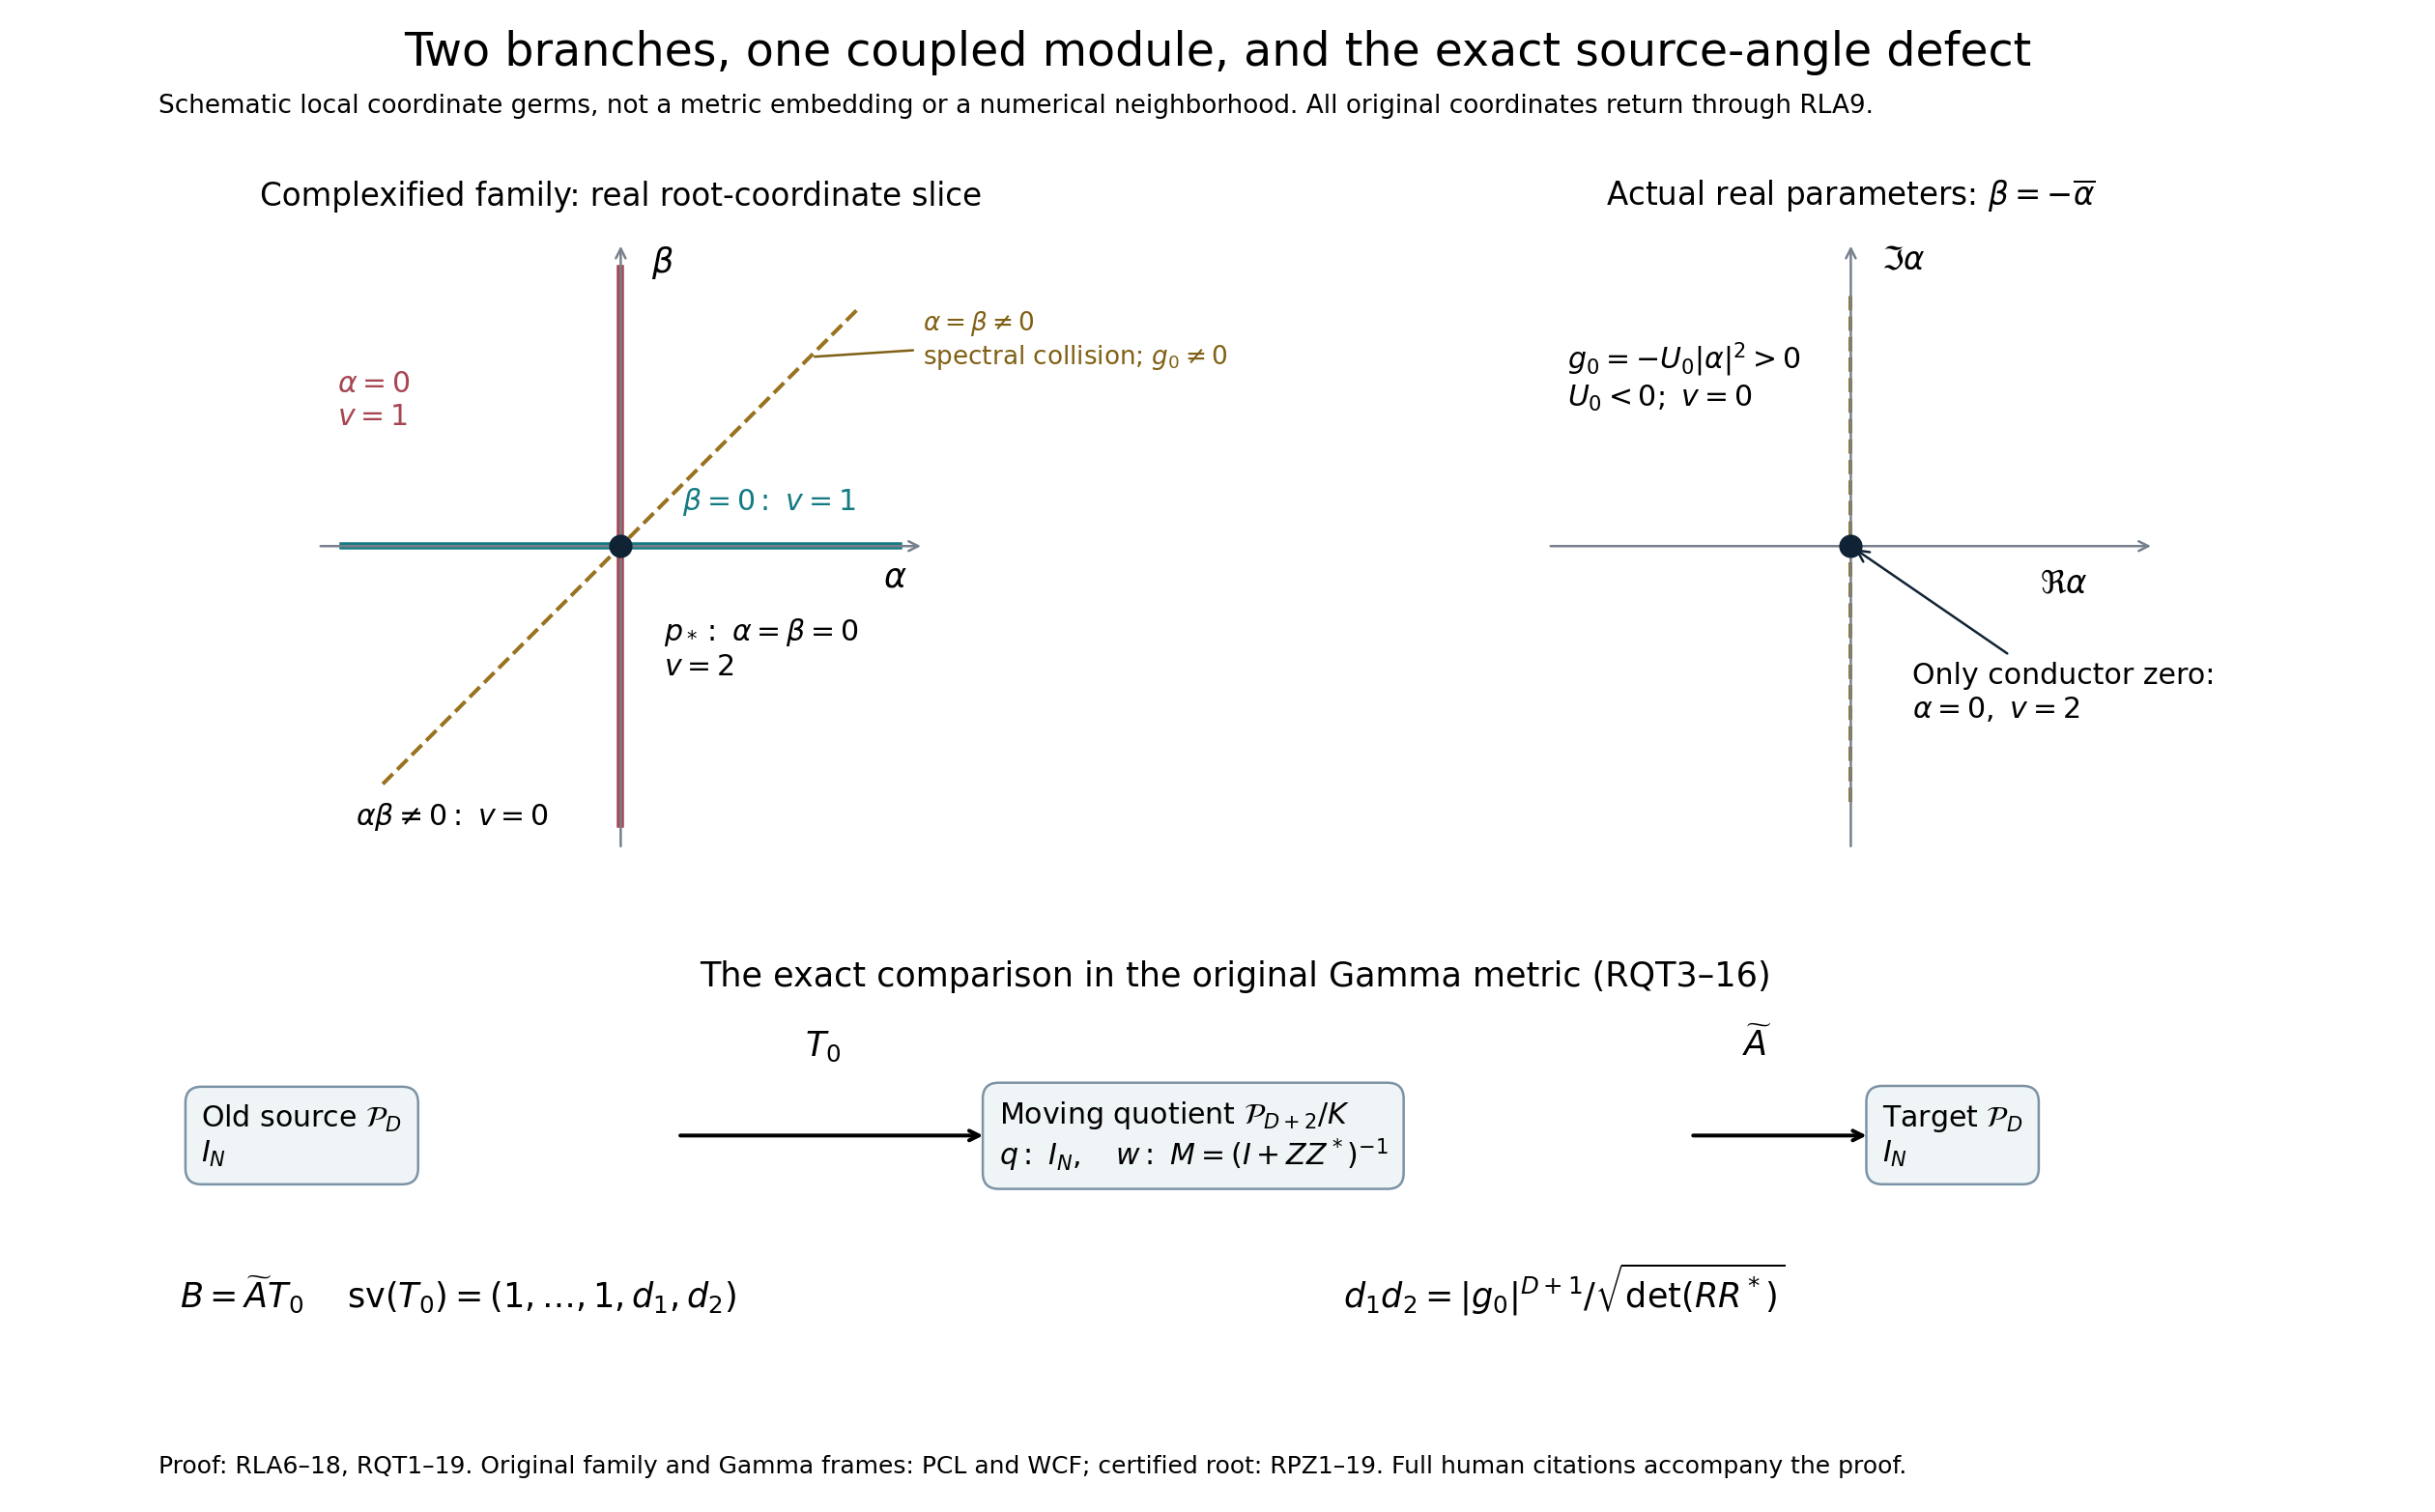
\includegraphics[width=.94\linewidth]{38_real_pair_local_object.png}
\caption{The two parameter branches are the exact coordinate axes of
RLA6--10; their coupled module, rather than an uncoupled sum, is
RLA14--18.  These are schematic local germs, not a metric drawing or
a certified numerical neighborhood.  The right chart is the actual
real parameter slice through the exact inverse RLA9.  A collision of
nonzero spectral roots does not make $g_0$ vanish.  RQT3--16 constructs
the bottom maps with the original Gamma metric: $T_0$ maps to
orthonormal quotient coordinates $q$, while the alternative coordinate
$w=M^{-1/2}q$ has Gram $M$.  Both angle sines and their full volume
correction are computed exactly.  Original family and metric:
\cite{PCLOriginal,WCF}; certified root: \cite{RPZ005}; complete
directional antecedent: \cite{RPD006}.}
\end{figure}\end{landscape}\clearpage
\begin{thebibliography}{99}
\bibitem{DLMF18Source} T. H. Koornwinder, R. Wong, R. Koekoek,
R. F. Swarttouw and W. P. Reinhardt,
NIST Digital Library of Mathematical Functions, Chapter 18,
\url{https://dlmf.nist.gov/18}, equations 18.19.8--9,
18.22.8 and 18.23.7. The original orthogonality and generating-function
dictionary is credited in WCF1--6; RS21--26 applies it with the complete
original centers, phases, Gamma mass and conductor inverse moments.


\bibitem{ES488} The Clankers, \emph{Erd\H{o}s--Straus project reader},
canonical 488-page edition, deposited source version 69,
\texttt{erdos\_straus\_project\_reader.tex}, theorem
\texttt{explicit-four-time-Jacobian-collision}, source lines
19484--19588. Source SHA-256:
\texttt{678b3f70ee7d2a6d00f6c588d7778e390118ab4743a5759612dbba6430984c78}.
The formal source uses the labels $\mathrm M,\mathrm N,\mathrm T,\mathrm E$.
The seven-point fibre and missing eighth factor-sign state are proved
here as an extension, rather than attributed to this reader.
 The complete original version-69 author source,
with the stated hash and byline, is included as
\nolinkurl{source_dependencies/ES_READER_V69.tex}.
\bibitem{PCLOriginal} Split-Zero programme,
\emph{The literal original conductor limit and an invertible pivot restriction},
\texttt{PCL\_COMPLETE.tex}, PCL1--16. Original supplied programme TeX;
the entire-period coefficient formula and prior positivity slice are
retained and cited at their use in OFM6--11. This is a programme source,
not an attribution of that construction to the classical human sources.



\href{https://github.com/KokunoYumeto/zeta-function-research-reader/blob/487253b5b01851da5b9b98af4e146fecf1fab902/workbenches/splitzero-tandem/continuations/20260919-native-conductor-coprimality/providers/PCL_COMPLETE.tex#L19}{Pinned public proof: PCL1--16}.
\bibitem{RPAC005} Split-Zero programme, result SZ-20260921-005, \nolinkurl{REAL_PAIR_ALL_CUTOFFS.tex}, RPAC1--15. \href{https://github.com/KokunoYumeto/zeta-function-research-reader/blob/0fd693c844aad9117e30ec447c59864a28af10f3/workbenches/splitzero-tandem/continuations/20260921-native-spectral-real-pair/005/REAL_PAIR_ALL_CUTOFFS.tex#L14}{Pinned complete public proof: RPAC1--15}.
\bibitem{RPCJ005} Split-Zero programme, result SZ-20260921-005, \nolinkurl{REAL_PAIR_COLLISION.tex}, RPCJ1--23. \href{https://github.com/KokunoYumeto/zeta-function-research-reader/blob/0fd693c844aad9117e30ec447c59864a28af10f3/workbenches/splitzero-tandem/continuations/20260921-native-spectral-real-pair/005/REAL_PAIR_COLLISION.tex#L20}{Pinned complete public proof: RPCJ1--23}.
\bibitem{RPD006} Split-Zero programme, result SZ-20260921-006, RPD1--30 and RPD12a. \href{https://github.com/KokunoYumeto/zeta-function-research-reader/blob/689a8f87e9c12b7a99b01b3123438c6751ee608f/workbenches/splitzero-tandem/continuations/20260921-directional-inverse-power/006/REAL_PAIR_DIRECTIONAL_GEOMETRY.tex#L43}{Pinned complete public proof: RPD1--30 and RPD12a}.
\bibitem{RPD31Source} Split-Zero programme, result SZ-20260921-006, RPD31. \href{https://github.com/KokunoYumeto/zeta-function-research-reader/blob/689a8f87e9c12b7a99b01b3123438c6751ee608f/workbenches/splitzero-tandem/continuations/20260921-directional-inverse-power/006/REAL_PAIR_DIRECTION_CERTIFICATE_BODY.tex#L22}{Pinned complete public proof: RPD31}.
\bibitem{RPE005} Split-Zero programme, result SZ-20260921-005, \nolinkurl{REAL_PAIR_ES_RETURN.tex}, RPE1--26. \href{https://github.com/KokunoYumeto/zeta-function-research-reader/blob/0fd693c844aad9117e30ec447c59864a28af10f3/workbenches/splitzero-tandem/continuations/20260921-native-spectral-real-pair/005/REAL_PAIR_ES_RETURN.tex#L18}{Pinned complete public proof: RPE1--26}.
\bibitem{RPZ005} Split-Zero programme, result SZ-20260921-005, \nolinkurl{REAL_PAIR_ZERO_BODY.tex}, RPZ1--19. \href{https://github.com/KokunoYumeto/zeta-function-research-reader/blob/0fd693c844aad9117e30ec447c59864a28af10f3/workbenches/splitzero-tandem/continuations/20260921-native-spectral-real-pair/005/REAL_PAIR_ZERO_BODY.tex#L18}{Pinned complete public proof: RPZ1--19}.
\bibitem{WCF} Split-Zero programme, \emph{A polynomial forward bound for
the full weighted conductor}, \texttt{WEIGHTED\_CONDUCTOR\_FORWARD.tex},
WCF1--6, source intake 17 September 2026. This source credits the
Meixner--Pollaczek dictionary to the NIST DLMF Chapter 18 by T. H. Koornwinder, R. Wong, R. Koekoek, R. F. Swarttouw and W. P. Reinhardt, equations
18.19.8--9, 18.22.8 and 18.23.7; its original phases and masses are
retained here, and no new orthogonality theorem is asserted.

\href{https://github.com/KokunoYumeto/zeta-function-research-reader/blob/5992ad50c0f2a06921f1fcaded7b4e38097c0739/workbenches/splitzero-tandem/continuations/20260920-original-kernel-mixed-determinants/providers/WEIGHTED_CONDUCTOR_FORWARD.tex#L28}{Pinned public proof: WCF1--6}.
\bibitem{human:arb2016} Fredrik Johansson,
\emph{Arb: Efficient Arbitrary-Precision Midpoint-Radius Interval Arithmetic},
original author source, arXiv:1611.02831v1 (9 November 2016),
\url{https://arxiv.org/abs/1611.02831v1}.
Source sections ``Features and example applications'', ``Radii and
magnitude bounds'' and ``Precision and bounds'' support the stated
inclusion arithmetic. The complete FPZ series-tail and zero-count proofs
are given here; they are not attributed to the software paper.
\end{thebibliography}
\end{document}
